\documentclass{article}
\usepackage[submission]{colm2026_conference}

\usepackage{microtype}
\usepackage{hyperref}
\usepackage{url}
\usepackage{booktabs}
\usepackage{graphicx}
\usepackage{amsmath}
\usepackage{amssymb}
\usepackage{tabularx}
\usepackage{caption}
\usepackage{subcaption}
\usepackage{enumitem}
\usepackage{placeins}
\usepackage{xcolor}
\usepackage{lineno}

%%%%% NEW MATH DEFINITIONS %%%%%

\usepackage{amsmath,amsfonts,bm}

% Mark sections of captions for referring to divisions of figures
\newcommand{\figleft}{{\em (Left)}}
\newcommand{\figcenter}{{\em (Center)}}
\newcommand{\figright}{{\em (Right)}}
\newcommand{\figtop}{{\em (Top)}}
\newcommand{\figbottom}{{\em (Bottom)}}
\newcommand{\captiona}{{\em (a)}}
\newcommand{\captionb}{{\em (b)}}
\newcommand{\captionc}{{\em (c)}}
\newcommand{\captiond}{{\em (d)}}

% Highlight a newly defined term
\newcommand{\newterm}[1]{{\bf #1}}


% Figure reference, lower-case.
\def\figref#1{figure~\ref{#1}}
% Figure reference, capital. For start of sentence
\def\Figref#1{Figure~\ref{#1}}
\def\twofigref#1#2{figures \ref{#1} and \ref{#2}}
\def\quadfigref#1#2#3#4{figures \ref{#1}, \ref{#2}, \ref{#3} and \ref{#4}}
% Section reference, lower-case.
\def\secref#1{section~\ref{#1}}
% Section reference, capital.
\def\Secref#1{Section~\ref{#1}}
% Reference to two sections.
\def\twosecrefs#1#2{sections \ref{#1} and \ref{#2}}
% Reference to three sections.
\def\secrefs#1#2#3{sections \ref{#1}, \ref{#2} and \ref{#3}}
% Reference to an equation, lower-case.
\def\eqref#1{equation~\ref{#1}}
% Reference to an equation, upper case
\def\Eqref#1{Equation~\ref{#1}}
% A raw reference to an equation---avoid using if possible
\def\plaineqref#1{\ref{#1}}
% Reference to a chapter, lower-case.
\def\chapref#1{chapter~\ref{#1}}
% Reference to an equation, upper case.
\def\Chapref#1{Chapter~\ref{#1}}
% Reference to a range of chapters
\def\rangechapref#1#2{chapters\ref{#1}--\ref{#2}}
% Reference to an algorithm, lower-case.
\def\algref#1{algorithm~\ref{#1}}
% Reference to an algorithm, upper case.
\def\Algref#1{Algorithm~\ref{#1}}
\def\twoalgref#1#2{algorithms \ref{#1} and \ref{#2}}
\def\Twoalgref#1#2{Algorithms \ref{#1} and \ref{#2}}
% Reference to a part, lower case
\def\partref#1{part~\ref{#1}}
% Reference to a part, upper case
\def\Partref#1{Part~\ref{#1}}
\def\twopartref#1#2{parts \ref{#1} and \ref{#2}}

\def\ceil#1{\lceil #1 \rceil}
\def\floor#1{\lfloor #1 \rfloor}
\def\1{\bm{1}}
\newcommand{\train}{\mathcal{D}}
\newcommand{\valid}{\mathcal{D_{\mathrm{valid}}}}
\newcommand{\test}{\mathcal{D_{\mathrm{test}}}}

\def\eps{{\epsilon}}


% Random variables
\def\reta{{\textnormal{$\eta$}}}
\def\ra{{\textnormal{a}}}
\def\rb{{\textnormal{b}}}
\def\rc{{\textnormal{c}}}
\def\rd{{\textnormal{d}}}
\def\re{{\textnormal{e}}}
\def\rf{{\textnormal{f}}}
\def\rg{{\textnormal{g}}}
\def\rh{{\textnormal{h}}}
\def\ri{{\textnormal{i}}}
\def\rj{{\textnormal{j}}}
\def\rk{{\textnormal{k}}}
\def\rl{{\textnormal{l}}}
% rm is already a command, just don't name any random variables m
\def\rn{{\textnormal{n}}}
\def\ro{{\textnormal{o}}}
\def\rp{{\textnormal{p}}}
\def\rq{{\textnormal{q}}}
\def\rr{{\textnormal{r}}}
\def\rs{{\textnormal{s}}}
\def\rt{{\textnormal{t}}}
\def\ru{{\textnormal{u}}}
\def\rv{{\textnormal{v}}}
\def\rw{{\textnormal{w}}}
\def\rx{{\textnormal{x}}}
\def\ry{{\textnormal{y}}}
\def\rz{{\textnormal{z}}}

% Random vectors
\def\rvepsilon{{\mathbf{\epsilon}}}
\def\rvtheta{{\mathbf{\theta}}}
\def\rva{{\mathbf{a}}}
\def\rvb{{\mathbf{b}}}
\def\rvc{{\mathbf{c}}}
\def\rvd{{\mathbf{d}}}
\def\rve{{\mathbf{e}}}
\def\rvf{{\mathbf{f}}}
\def\rvg{{\mathbf{g}}}
\def\rvh{{\mathbf{h}}}
\def\rvu{{\mathbf{i}}}
\def\rvj{{\mathbf{j}}}
\def\rvk{{\mathbf{k}}}
\def\rvl{{\mathbf{l}}}
\def\rvm{{\mathbf{m}}}
\def\rvn{{\mathbf{n}}}
\def\rvo{{\mathbf{o}}}
\def\rvp{{\mathbf{p}}}
\def\rvq{{\mathbf{q}}}
\def\rvr{{\mathbf{r}}}
\def\rvs{{\mathbf{s}}}
\def\rvt{{\mathbf{t}}}
\def\rvu{{\mathbf{u}}}
\def\rvv{{\mathbf{v}}}
\def\rvw{{\mathbf{w}}}
\def\rvx{{\mathbf{x}}}
\def\rvy{{\mathbf{y}}}
\def\rvz{{\mathbf{z}}}

% Elements of random vectors
\def\erva{{\textnormal{a}}}
\def\ervb{{\textnormal{b}}}
\def\ervc{{\textnormal{c}}}
\def\ervd{{\textnormal{d}}}
\def\erve{{\textnormal{e}}}
\def\ervf{{\textnormal{f}}}
\def\ervg{{\textnormal{g}}}
\def\ervh{{\textnormal{h}}}
\def\ervi{{\textnormal{i}}}
\def\ervj{{\textnormal{j}}}
\def\ervk{{\textnormal{k}}}
\def\ervl{{\textnormal{l}}}
\def\ervm{{\textnormal{m}}}
\def\ervn{{\textnormal{n}}}
\def\ervo{{\textnormal{o}}}
\def\ervp{{\textnormal{p}}}
\def\ervq{{\textnormal{q}}}
\def\ervr{{\textnormal{r}}}
\def\ervs{{\textnormal{s}}}
\def\ervt{{\textnormal{t}}}
\def\ervu{{\textnormal{u}}}
\def\ervv{{\textnormal{v}}}
\def\ervw{{\textnormal{w}}}
\def\ervx{{\textnormal{x}}}
\def\ervy{{\textnormal{y}}}
\def\ervz{{\textnormal{z}}}

% Random matrices
\def\rmA{{\mathbf{A}}}
\def\rmB{{\mathbf{B}}}
\def\rmC{{\mathbf{C}}}
\def\rmD{{\mathbf{D}}}
\def\rmE{{\mathbf{E}}}
\def\rmF{{\mathbf{F}}}
\def\rmG{{\mathbf{G}}}
\def\rmH{{\mathbf{H}}}
\def\rmI{{\mathbf{I}}}
\def\rmJ{{\mathbf{J}}}
\def\rmK{{\mathbf{K}}}
\def\rmL{{\mathbf{L}}}
\def\rmM{{\mathbf{M}}}
\def\rmN{{\mathbf{N}}}
\def\rmO{{\mathbf{O}}}
\def\rmP{{\mathbf{P}}}
\def\rmQ{{\mathbf{Q}}}
\def\rmR{{\mathbf{R}}}
\def\rmS{{\mathbf{S}}}
\def\rmT{{\mathbf{T}}}
\def\rmU{{\mathbf{U}}}
\def\rmV{{\mathbf{V}}}
\def\rmW{{\mathbf{W}}}
\def\rmX{{\mathbf{X}}}
\def\rmY{{\mathbf{Y}}}
\def\rmZ{{\mathbf{Z}}}

% Elements of random matrices
\def\ermA{{\textnormal{A}}}
\def\ermB{{\textnormal{B}}}
\def\ermC{{\textnormal{C}}}
\def\ermD{{\textnormal{D}}}
\def\ermE{{\textnormal{E}}}
\def\ermF{{\textnormal{F}}}
\def\ermG{{\textnormal{G}}}
\def\ermH{{\textnormal{H}}}
\def\ermI{{\textnormal{I}}}
\def\ermJ{{\textnormal{J}}}
\def\ermK{{\textnormal{K}}}
\def\ermL{{\textnormal{L}}}
\def\ermM{{\textnormal{M}}}
\def\ermN{{\textnormal{N}}}
\def\ermO{{\textnormal{O}}}
\def\ermP{{\textnormal{P}}}
\def\ermQ{{\textnormal{Q}}}
\def\ermR{{\textnormal{R}}}
\def\ermS{{\textnormal{S}}}
\def\ermT{{\textnormal{T}}}
\def\ermU{{\textnormal{U}}}
\def\ermV{{\textnormal{V}}}
\def\ermW{{\textnormal{W}}}
\def\ermX{{\textnormal{X}}}
\def\ermY{{\textnormal{Y}}}
\def\ermZ{{\textnormal{Z}}}

% Vectors
\def\vzero{{\bm{0}}}
\def\vone{{\bm{1}}}
\def\vmu{{\bm{\mu}}}
\def\vtheta{{\bm{\theta}}}
\def\va{{\bm{a}}}
\def\vb{{\bm{b}}}
\def\vc{{\bm{c}}}
\def\vd{{\bm{d}}}
\def\ve{{\bm{e}}}
\def\vf{{\bm{f}}}
\def\vg{{\bm{g}}}
\def\vh{{\bm{h}}}
\def\vi{{\bm{i}}}
\def\vj{{\bm{j}}}
\def\vk{{\bm{k}}}
\def\vl{{\bm{l}}}
\def\vm{{\bm{m}}}
\def\vn{{\bm{n}}}
\def\vo{{\bm{o}}}
\def\vp{{\bm{p}}}
\def\vq{{\bm{q}}}
\def\vr{{\bm{r}}}
\def\vs{{\bm{s}}}
\def\vt{{\bm{t}}}
\def\vu{{\bm{u}}}
\def\vv{{\bm{v}}}
\def\vw{{\bm{w}}}
\def\vx{{\bm{x}}}
\def\vy{{\bm{y}}}
\def\vz{{\bm{z}}}

% Elements of vectors
\def\evalpha{{\alpha}}
\def\evbeta{{\beta}}
\def\evepsilon{{\epsilon}}
\def\evlambda{{\lambda}}
\def\evomega{{\omega}}
\def\evmu{{\mu}}
\def\evpsi{{\psi}}
\def\evsigma{{\sigma}}
\def\evtheta{{\theta}}
\def\eva{{a}}
\def\evb{{b}}
\def\evc{{c}}
\def\evd{{d}}
\def\eve{{e}}
\def\evf{{f}}
\def\evg{{g}}
\def\evh{{h}}
\def\evi{{i}}
\def\evj{{j}}
\def\evk{{k}}
\def\evl{{l}}
\def\evm{{m}}
\def\evn{{n}}
\def\evo{{o}}
\def\evp{{p}}
\def\evq{{q}}
\def\evr{{r}}
\def\evs{{s}}
\def\evt{{t}}
\def\evu{{u}}
\def\evv{{v}}
\def\evw{{w}}
\def\evx{{x}}
\def\evy{{y}}
\def\evz{{z}}

% Matrix
\def\mA{{\bm{A}}}
\def\mB{{\bm{B}}}
\def\mC{{\bm{C}}}
\def\mD{{\bm{D}}}
\def\mE{{\bm{E}}}
\def\mF{{\bm{F}}}
\def\mG{{\bm{G}}}
\def\mH{{\bm{H}}}
\def\mI{{\bm{I}}}
\def\mJ{{\bm{J}}}
\def\mK{{\bm{K}}}
\def\mL{{\bm{L}}}
\def\mM{{\bm{M}}}
\def\mN{{\bm{N}}}
\def\mO{{\bm{O}}}
\def\mP{{\bm{P}}}
\def\mQ{{\bm{Q}}}
\def\mR{{\bm{R}}}
\def\mS{{\bm{S}}}
\def\mT{{\bm{T}}}
\def\mU{{\bm{U}}}
\def\mV{{\bm{V}}}
\def\mW{{\bm{W}}}
\def\mX{{\bm{X}}}
\def\mY{{\bm{Y}}}
\def\mZ{{\bm{Z}}}
\def\mBeta{{\bm{\beta}}}
\def\mPhi{{\bm{\Phi}}}
\def\mLambda{{\bm{\Lambda}}}
\def\mSigma{{\bm{\Sigma}}}

% Tensor
\DeclareMathAlphabet{\mathsfit}{\encodingdefault}{\sfdefault}{m}{sl}
\SetMathAlphabet{\mathsfit}{bold}{\encodingdefault}{\sfdefault}{bx}{n}
\newcommand{\tens}[1]{\bm{\mathsfit{#1}}}
\def\tA{{\tens{A}}}
\def\tB{{\tens{B}}}
\def\tC{{\tens{C}}}
\def\tD{{\tens{D}}}
\def\tE{{\tens{E}}}
\def\tF{{\tens{F}}}
\def\tG{{\tens{G}}}
\def\tH{{\tens{H}}}
\def\tI{{\tens{I}}}
\def\tJ{{\tens{J}}}
\def\tK{{\tens{K}}}
\def\tL{{\tens{L}}}
\def\tM{{\tens{M}}}
\def\tN{{\tens{N}}}
\def\tO{{\tens{O}}}
\def\tP{{\tens{P}}}
\def\tQ{{\tens{Q}}}
\def\tR{{\tens{R}}}
\def\tS{{\tens{S}}}
\def\tT{{\tens{T}}}
\def\tU{{\tens{U}}}
\def\tV{{\tens{V}}}
\def\tW{{\tens{W}}}
\def\tX{{\tens{X}}}
\def\tY{{\tens{Y}}}
\def\tZ{{\tens{Z}}}


% Graph
\def\gA{{\mathcal{A}}}
\def\gB{{\mathcal{B}}}
\def\gC{{\mathcal{C}}}
\def\gD{{\mathcal{D}}}
\def\gE{{\mathcal{E}}}
\def\gF{{\mathcal{F}}}
\def\gG{{\mathcal{G}}}
\def\gH{{\mathcal{H}}}
\def\gI{{\mathcal{I}}}
\def\gJ{{\mathcal{J}}}
\def\gK{{\mathcal{K}}}
\def\gL{{\mathcal{L}}}
\def\gM{{\mathcal{M}}}
\def\gN{{\mathcal{N}}}
\def\gO{{\mathcal{O}}}
\def\gP{{\mathcal{P}}}
\def\gQ{{\mathcal{Q}}}
\def\gR{{\mathcal{R}}}
\def\gS{{\mathcal{S}}}
\def\gT{{\mathcal{T}}}
\def\gU{{\mathcal{U}}}
\def\gV{{\mathcal{V}}}
\def\gW{{\mathcal{W}}}
\def\gX{{\mathcal{X}}}
\def\gY{{\mathcal{Y}}}
\def\gZ{{\mathcal{Z}}}

% Sets
\def\sA{{\mathbb{A}}}
\def\sB{{\mathbb{B}}}
\def\sC{{\mathbb{C}}}
\def\sD{{\mathbb{D}}}
% Don't use a set called E, because this would be the same as our symbol
% for expectation.
\def\sF{{\mathbb{F}}}
\def\sG{{\mathbb{G}}}
\def\sH{{\mathbb{H}}}
\def\sI{{\mathbb{I}}}
\def\sJ{{\mathbb{J}}}
\def\sK{{\mathbb{K}}}
\def\sL{{\mathbb{L}}}
\def\sM{{\mathbb{M}}}
\def\sN{{\mathbb{N}}}
\def\sO{{\mathbb{O}}}
\def\sP{{\mathbb{P}}}
\def\sQ{{\mathbb{Q}}}
\def\sR{{\mathbb{R}}}
\def\sS{{\mathbb{S}}}
\def\sT{{\mathbb{T}}}
\def\sU{{\mathbb{U}}}
\def\sV{{\mathbb{V}}}
\def\sW{{\mathbb{W}}}
\def\sX{{\mathbb{X}}}
\def\sY{{\mathbb{Y}}}
\def\sZ{{\mathbb{Z}}}

% Entries of a matrix
\def\emLambda{{\Lambda}}
\def\emA{{A}}
\def\emB{{B}}
\def\emC{{C}}
\def\emD{{D}}
\def\emE{{E}}
\def\emF{{F}}
\def\emG{{G}}
\def\emH{{H}}
\def\emI{{I}}
\def\emJ{{J}}
\def\emK{{K}}
\def\emL{{L}}
\def\emM{{M}}
\def\emN{{N}}
\def\emO{{O}}
\def\emP{{P}}
\def\emQ{{Q}}
\def\emR{{R}}
\def\emS{{S}}
\def\emT{{T}}
\def\emU{{U}}
\def\emV{{V}}
\def\emW{{W}}
\def\emX{{X}}
\def\emY{{Y}}
\def\emZ{{Z}}
\def\emSigma{{\Sigma}}

% entries of a tensor
% Same font as tensor, without \bm wrapper
\newcommand{\etens}[1]{\mathsfit{#1}}
\def\etLambda{{\etens{\Lambda}}}
\def\etA{{\etens{A}}}
\def\etB{{\etens{B}}}
\def\etC{{\etens{C}}}
\def\etD{{\etens{D}}}
\def\etE{{\etens{E}}}
\def\etF{{\etens{F}}}
\def\etG{{\etens{G}}}
\def\etH{{\etens{H}}}
\def\etI{{\etens{I}}}
\def\etJ{{\etens{J}}}
\def\etK{{\etens{K}}}
\def\etL{{\etens{L}}}
\def\etM{{\etens{M}}}
\def\etN{{\etens{N}}}
\def\etO{{\etens{O}}}
\def\etP{{\etens{P}}}
\def\etQ{{\etens{Q}}}
\def\etR{{\etens{R}}}
\def\etS{{\etens{S}}}
\def\etT{{\etens{T}}}
\def\etU{{\etens{U}}}
\def\etV{{\etens{V}}}
\def\etW{{\etens{W}}}
\def\etX{{\etens{X}}}
\def\etY{{\etens{Y}}}
\def\etZ{{\etens{Z}}}

% The true underlying data generating distribution
\newcommand{\pdata}{p_{\rm{data}}}
% The empirical distribution defined by the training set
\newcommand{\ptrain}{\hat{p}_{\rm{data}}}
\newcommand{\Ptrain}{\hat{P}_{\rm{data}}}
% The model distribution
\newcommand{\pmodel}{p_{\rm{model}}}
\newcommand{\Pmodel}{P_{\rm{model}}}
\newcommand{\ptildemodel}{\tilde{p}_{\rm{model}}}
% Stochastic autoencoder distributions
\newcommand{\pencode}{p_{\rm{encoder}}}
\newcommand{\pdecode}{p_{\rm{decoder}}}
\newcommand{\precons}{p_{\rm{reconstruct}}}

\newcommand{\laplace}{\mathrm{Laplace}} % Laplace distribution

\newcommand{\E}{\mathbb{E}}
\newcommand{\Ls}{\mathcal{L}}
\newcommand{\R}{\mathbb{R}}
\newcommand{\emp}{\tilde{p}}
\newcommand{\lr}{\alpha}
\newcommand{\reg}{\lambda}
\newcommand{\rect}{\mathrm{rectifier}}
\newcommand{\softmax}{\mathrm{softmax}}
\newcommand{\sigmoid}{\sigma}
\newcommand{\softplus}{\zeta}
\newcommand{\KL}{D_{\mathrm{KL}}}
\newcommand{\Var}{\mathrm{Var}}
\newcommand{\standarderror}{\mathrm{SE}}
\newcommand{\Cov}{\mathrm{Cov}}
% Wolfram Mathworld says $L^2$ is for function spaces and $\ell^2$ is for vectors
% But then they seem to use $L^2$ for vectors throughout the site, and so does
% wikipedia.
\newcommand{\normlzero}{L^0}
\newcommand{\normlone}{L^1}
\newcommand{\normltwo}{L^2}
\newcommand{\normlp}{L^p}
\newcommand{\normmax}{L^\infty}

\newcommand{\parents}{Pa} % See usage in notation.tex. Chosen to match Daphne's book.

\DeclareMathOperator*{\argmax}{arg\,max}
\DeclareMathOperator*{\argmin}{arg\,min}

\DeclareMathOperator{\sign}{sign}
\DeclareMathOperator{\Tr}{Tr}
\let\ab\allowbreak

\newcommand{\ArcPromptCount}{195}
\newcommand{\CsqaPromptCount}{794}
\newcommand{\ExemplarCount}{3}
\newcommand{\FinalLayerTieCount}{45}
\newcommand{\MainPromptCount}{989}
\newcommand{\MaxMedianDeltaTwoFifty}{0.19}
\newcommand{\MaxWriteAfterDTwo}{69\%}
\newcommand{\MergedRunId}{paper\_merged\_9x1000\_20260330T122258Z}
\newcommand{\MinMedianDeltaTwoFifty}{0.09}
\newcommand{\MinWriteAfterDTwo}{38\%}
\newcommand{\MmluPromptCount}{11}
\newcommand{\NormalizedGapExcludedCount}{45}
\newcommand{\PaperPromptCount}{1000}
\newcommand{\PooledDeltaTwentyFiftyHigh}{0.15}
\newcommand{\PooledDeltaTwentyFiftyLow}{0.13}
\newcommand{\PooledDeltaTwentyOneHigh}{0.10}
\newcommand{\PooledDeltaTwentyOneLow}{0.08}
\newcommand{\PooledDeltaTwoFiftyPct}{15\%}
\newcommand{\PooledDeltaTwoOnePct}{9\%}
\newcommand{\PooledMedianDFifty}{0.94}
\newcommand{\PooledMedianDOne}{0.89}
\newcommand{\PooledMedianDTwo}{0.70}
\newcommand{\PooledMedianDeltaTwentyFifty}{0.15}
\newcommand{\PooledMedianDeltaTwentyOne}{0.09}
\newcommand{\PooledWriteAfterDOne}{29\%}
\newcommand{\PooledWriteAfterDTwo}{50\%}
\newcommand{\PooledWriteLastTwenty}{29\%}


\graphicspath{{figures/}}
\definecolor{darkblue}{rgb}{0, 0, 0.5}
\hypersetup{colorlinks=true, citecolor=darkblue, linkcolor=darkblue, urlcolor=darkblue}

\title{Persistent Contenders, Late Margins: Winner Isolation Across Model Depth}
\author{Anonymous Authors}

\begin{document}
\ifcolmsubmission
\linenumbers
\fi
\maketitle

\begin{abstract}
Layerwise winner analysis depends on how early and late events are defined. We revisit an existing nine-model multiple-choice cache using exact-option continuation scoring and replace an asymmetric first-hit-versus-persistent comparison with a fully persistence-based one. For each prompt, we measure the first layer after which the final winner never leaves the top-2, the first layer after which it remains top-1, and the first layer after which its winner-runner gap never again falls below half of its final value. Across the tested panel, the pooled median normalized lag $\Delta_{250}=d_{50}-d_2$ is \PooledMedianDeltaTwentyFifty{} with a 95\% bootstrap interval of [\PooledDeltaTwentyFiftyLow{}, \PooledDeltaTwentyFiftyHigh{}]. The median share of winner-gap growth that occurs after $d_2$ is \PooledWriteAfterDTwo{}, which means substantial separation is still written after persistent contender status is already in place. These results are limited to exact-option score dynamics in the nine tested models and do not claim answer-format invariance, a hidden-state mechanism, or universality.
\end{abstract}

\section{Introduction}

A final answer compresses a depth-wise process into one surface choice. The older draft in this repository tried to describe that process by comparing a weak first-hit event to stronger forever-after events. That comparison was asymmetric, so part of the reported lag could come from the metric definitions rather than from the score dynamics themselves.

This paper replaces that center with a fully persistence-based one. Under exact-option continuation scoring, we ask when the eventual winner first becomes a contender that never leaves the top-2 again, when it becomes the top-1 option for the rest of depth, and when it finally acquires a winner-runner gap that never again drops below half of its final value. Figure~\ref{fig:pooled-cdfs} shows those three persistent depths in one view.

The claim is deliberately narrow. We study only cached exact-option score trajectories for nine tested instruction-tuned open-weight models. We do not use this analysis to claim answer-format invariance, a hidden-state mechanism, or universality beyond the tested panel. Within that scope, the central pattern is consistent: the lag from persistent contender status to persistent decisive margin is typically nontrivial.

\section{Setup and corrected operationalization}

The analysis uses the existing merged run \texttt{\MergedRunId} and performs zero new inference. The tested panel contains nine instruction-tuned open-weight checkpoints from the Qwen 2.5 Instruct, Gemma 2 IT, and Llama families \citep{qwen25card,gemma2card,llama3herd}. In total, the cache covers \PaperPromptCount{} prompts: \ArcPromptCount{} ARC-Challenge prompts \citep{clark2018arc}, \CsqaPromptCount{} CommonsenseQA prompts \citep{talmor2019commonsenseqa}, and a small \MmluPromptCount{}-question MMLU Abstract Algebra slice \citep{hendrycks2021mmlu} that we keep out of the main narrative.

The main paper uses only the exact-option readout with identity option ordering. For each model, prompt, layer, and answer option, the restored cache stores the option score along the exact continuation string for that answer. We therefore analyze winner dynamics directly in exact-option decision space without rerunning models, generating new completions, or adding external probes.

Let $w^\star$ be the final-layer winner, defined as the highest-scoring option at the final layer with deterministic tie-breaking by canonical option order. At each layer $\ell$, let $\mathrm{rank}_\ell(w^\star)$ be the rank of that final winner among all options, with rank 1 best. Let $g_\ell$ be the final winner's score gap over the strongest competing option at layer $\ell$, and let $g_L$ be the final-layer gap. When $g_L > 0$, we normalize by the final gap and write $m_\ell = g_\ell / g_L$.

The corrected persistent depths are:
\begin{align}
d_2 &= \min \{\ell : \mathrm{rank}_t(w^\star) \le 2 \text{ for all } t \ge \ell\}, \\
d_1 &= \min \{\ell : \mathrm{rank}_t(w^\star) = 1 \text{ for all } t \ge \ell\}, \\
d_{50} &= \min \{\ell : m_t \ge 0.50 \text{ for all } t \ge \ell\}.
\end{align}
In words, $d_2$ is the first layer after which the final winner never leaves the top-2 again, $d_1$ is the first layer after which it remains top-1 for the rest of depth, and $d_{50}$ is the first layer after which its winner-runner gap never again falls below half of its final value.

The main lag objects are $\Delta_{21} = d_1 - d_2$ and $\Delta_{250} = d_{50} - d_2$. We also track where winner-gap growth is added. For $\ell > 0$, let $\Delta g_\ell = g_\ell - g_{\ell-1}$ and $\mathrm{positive\_write}_\ell = \max(\Delta g_\ell, 0)$. From these increments we compute the share written after $d_2$, the share written after $d_1$, and the share written in the last 20\% of normalized depth. The old first-hit-versus-persistent comparison is not used anywhere in this paper because it was asymmetric by construction.


\begin{figure*}[t]
\centering
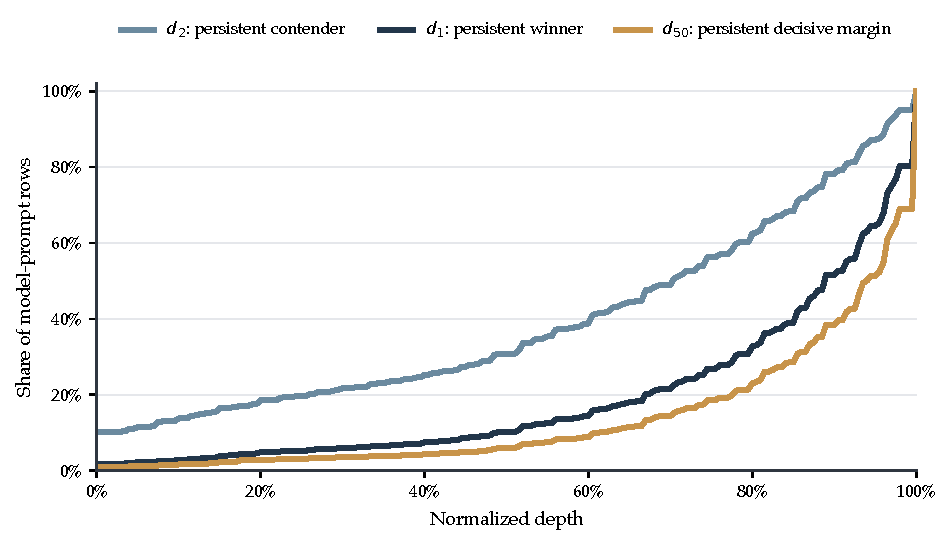
\includegraphics[width=\textwidth]{figure1_pooled_cdfs.pdf}
\caption{\textbf{Pooled persistence CDFs for the corrected operationalization.} Each curve is an empirical CDF over exact-option model-prompt rows. The persistent contender depth $d_2$ arrives earliest, the persistent winner depth $d_1$ arrives later, and the persistent 50\% final-gap depth $d_{50}$ arrives later still. This is the corrected paper center: all three events are defined with the same persistence logic.}
\label{fig:pooled-cdfs}
\end{figure*}

\section{Main results}

Figure~\ref{fig:pooled-cdfs} shows the corrected paper center in one view. The pooled CDF for $d_2$ sits left of the pooled CDF for $d_1$, which in turn sits left of the pooled CDF for $d_{50}$. In normalized depth, the pooled medians are \PooledMedianDTwo{} for $d_2$, \PooledMedianDOne{} for $d_1$, and \PooledMedianDFifty{} for $d_{50}$.

The main lag object is $\Delta_{250} = d_{50} - d_2$. Its pooled median is \PooledMedianDeltaTwentyFifty{}, with a 95\% bootstrap interval of [\PooledDeltaTwentyFiftyLow{}, \PooledDeltaTwentyFiftyHigh{}]. The smaller persistent-rank lag $\Delta_{21} = d_1 - d_2$ is also nontrivial in the pooled data, with median \PooledMedianDeltaTwentyOne{} and 95\% interval [\PooledDeltaTwentyOneLow{}, \PooledDeltaTwentyOneHigh{}]. Figure~\ref{fig:lag-summary} shows both quantities by model.

Because $d_2 \le d_1 \le d_{50}$ is partly nested by construction on valid rows, sign alone is not the main result. The substantive result is magnitude. A median $\Delta_{250}$ of \PooledDeltaTwoFiftyPct{} means that, after the final winner has already become a persistent contender, the model typically uses about another 15\% of normalized depth before it acquires a persistent decisive margin.


\begin{figure*}[t]
\centering
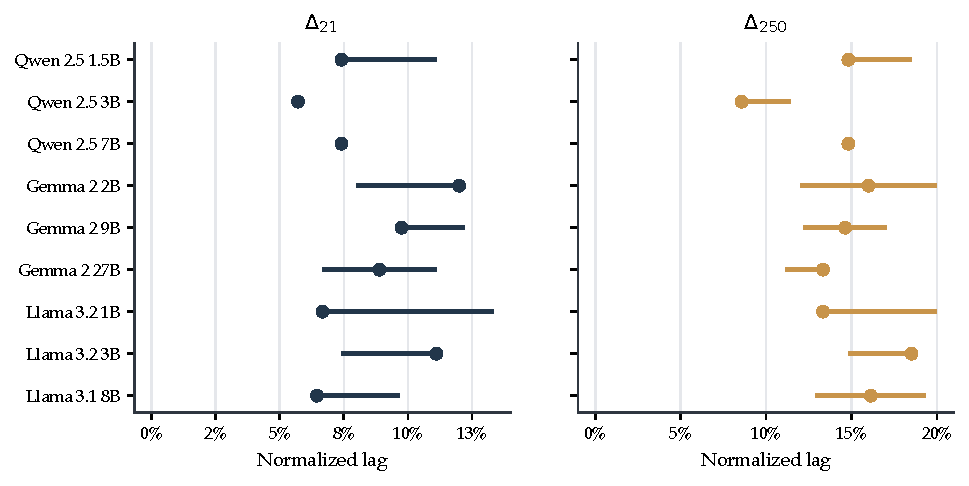
\includegraphics[width=\textwidth]{figure2_lag_summary.pdf}
\caption{\textbf{Model-level lag magnitudes under the corrected persistence rules.} Points are model medians and horizontal intervals are 95\% prompt-bootstrap confidence intervals in normalized depth. Because $d_2 \le d_1 \le d_{50}$ is partly nested by construction, the key result is the size of $\Delta_{21}$ and $\Delta_{250}$, not just that they are nonnegative.}
\label{fig:lag-summary}
\end{figure*}

\begin{figure*}[t]
\centering
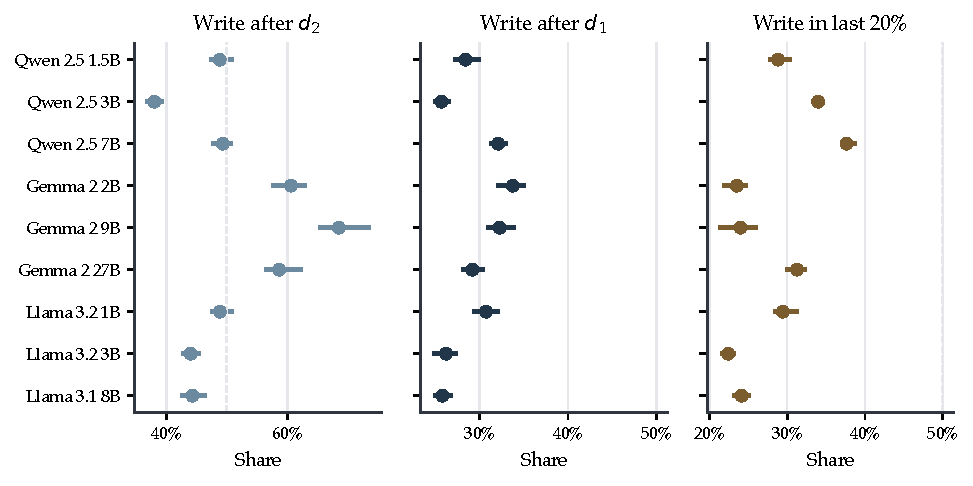
\includegraphics[width=\textwidth]{figure3_late_write.pdf}
\caption{\textbf{Late-write concentration after persistent contender and winner entry.} Each point is a model median and each horizontal interval is a 95\% prompt-bootstrap confidence interval. The left panel is the main complement to the lag plot: it measures how much winner-runner separation is still written after the final winner has already entered stable top-2 status.}
\label{fig:latewrite}
\end{figure*}

\begin{table}[t]
\centering
\small
\begin{tabularx}{\linewidth}{@{}lX@{}}
\toprule
\textbf{Aspect} & \textbf{Configuration}\\
\midrule
Models & Nine tested instruction-tuned open-weight checkpoints from the Qwen 2.5 Instruct, Gemma 2 IT, and Llama Instruct families. \\
Data source & Existing exact-option per-layer cache only. No new inference, no new completions, and no new model downloads. \\
Primary readout & \texttt{semantic\_exact} with identity option ordering. \\
Persistent depths & $d_2$: first layer after which the eventual winner never leaves the top-2; $d_1$: first layer after which it stays top-1; $d_{50}$: first layer after which the winner gap never falls below 50\% of its final gap. \\
Primary lags & $\Delta_{21}=d_1-d_2$ and $\Delta_{250}=d_{50}-d_2$. \\
Late-write metrics & Share of winner-gap growth written after $d_2$, after $d_1$, and in the final 20\% of depth. \\
\bottomrule
\end{tabularx}

\caption{\textbf{Design summary for the corrected v3 analysis.}}
\label{tab:design}
\end{table}

\section{Model heterogeneity}

The lag is common within the tested panel, but its size is not constant. Figure~\ref{fig:lag-summary} shows that model medians for $\Delta_{250}$ range from \MinMedianDeltaTwoFifty{} to \MaxMedianDeltaTwoFifty{} in normalized depth. Figure~\ref{fig:latewrite} shows a comparable spread in late-write concentration: model medians for write share after $d_2$ range from \MinWriteAfterDTwo{} to \MaxWriteAfterDTwo{}.

The late-write figure is the key complement to the lag figure. A nontrivial lag can arise partly from nested persistent events, but a large write share after $d_2$ means that substantial additional winner-runner separation is still being written after the final winner has already entered stable top-2 status. In the pooled data, the median write share after $d_2$ is \PooledWriteAfterDTwo{}, the median write share after $d_1$ is \PooledWriteAfterDOne{}, and the median write share in the last 20\% of depth is \PooledWriteLastTwenty{}.

The appendix summary table keeps the supporting descriptive numbers in one place: model-level medians and confidence intervals for $\Delta_{250}$, plus the median write share after $d_2$. That appendix material is descriptive only. The main paper argument remains about lag magnitude, late-write concentration, and heterogeneity across the tested panel.


\begin{figure*}[t]
\centering
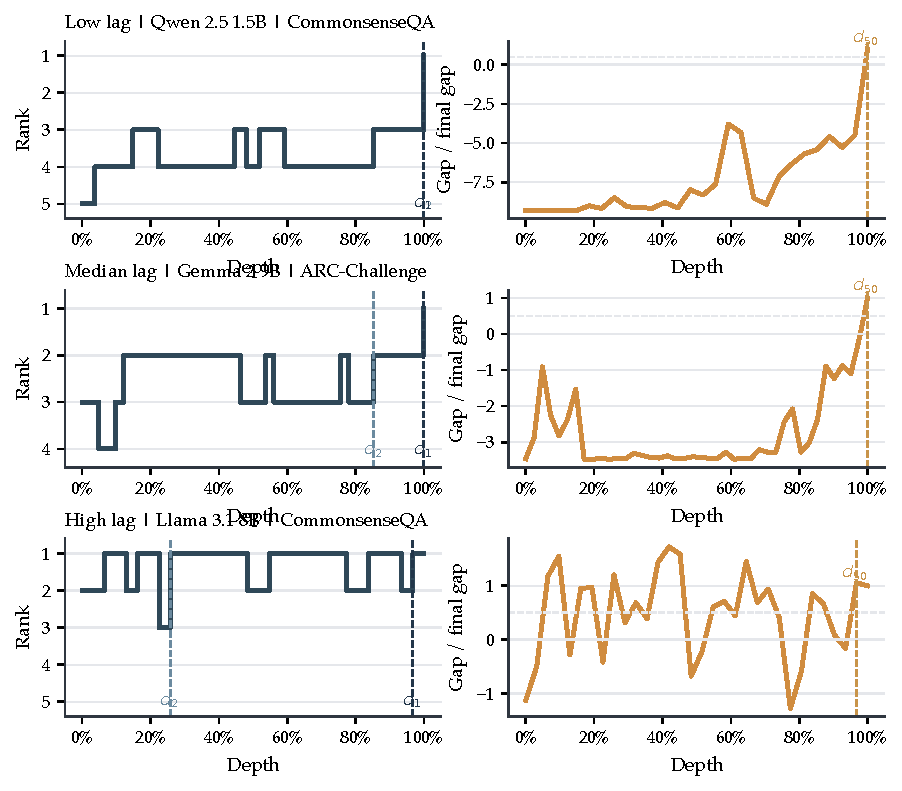
\includegraphics[width=\textwidth]{figure4_exemplars.pdf}
\caption{\textbf{Illustrative, algorithmically selected trajectories.} The three rows are the valid exact-option identity cases whose normalized $\Delta_{250}$ values are closest to the pooled 10th, 50th, and 90th percentiles, with ties broken by source row index, then model name, then example id. The left panel shows final-winner rank across depth, and the right panel shows the winner-runner gap normalized by its final value.}
\label{fig:exemplars}
\end{figure*}

\begin{table}[t]
\centering
\small
\begin{tabular}{@{}lccc@{}}
\toprule
Model & Median $\Delta_{21}$ & Median $\Delta_{250}$ & Median write share after $d_2$ \\
\midrule
Qwen 2.5 1.5B & 0.07 & 0.15 & 49\% \\
Qwen 2.5 3B & 0.06 & 0.09 & 38\% \\
Qwen 2.5 7B & 0.07 & 0.15 & 49\% \\
Gemma 2 2B & 0.12 & 0.16 & 61\% \\
Gemma 2 9B & 0.10 & 0.15 & 69\% \\
Gemma 2 27B & 0.09 & 0.13 & 59\% \\
Llama 3.2 1B & 0.07 & 0.13 & 49\% \\
Llama 3.2 3B & 0.11 & 0.19 & 44\% \\
Llama 3.1 8B & 0.06 & 0.16 & 44\% \\
\bottomrule
\end{tabular}

\caption{\textbf{Compact model summary for the corrected analysis.}}
\label{tab:model-summary}
\end{table}

\section{Limitations}

The scope of the paper is intentionally narrow. The analysis concerns exact-option score dynamics only, for nine tested models, under one primary readout and one primary option ordering. It is not a claim about hidden states in general, not a claim about semantic invariance across answer formats, and not a causal explanation of how the networks decide.

Some of the reported lags are constrained to be nonnegative by the nesting of the persistence definitions. That is why the paper emphasizes lag magnitude and late-write concentration rather than sign alone. We also keep the small MMLU slice out of the main narrative because its count is too small to support strong benchmark-level claims.

Alternate answer-format controls were heterogeneous in evaluability and sometimes in final winner identity. We therefore treat them only as sensitivity context and not as primary evidence for the main claim. No robustness or invariance claim is made from those controls.

\section{Conclusion}

This paper studies one narrow object: exact-option continuation scores in nine tested models. Under that readout, the final winner typically becomes a persistent contender before it acquires a persistent decisive margin. The same cache also shows that substantial winner-runner separation is often written after persistent contender status has already been reached.

The conclusion stops there. Controls are heterogeneous and therefore not used as primary evidence, the paper does not claim a hidden-state mechanism, and the result should not be read as a universal statement about all language models. Within the tested panel and this persistence-based operationalization, however, the lag from persistent contender to persistent margin is real, measurable, and often substantial.


\bibliographystyle{colm2026_conference}
\bibliography{references}

\onecolumn
\appendix
\section{Supplementary material}

\subsection{Reproducibility statement}

The v3 workspace is a zero-new-inference reanalysis. It reads an existing merged run manifest, resolves raw exact-option cache bundles by cache key, computes the corrected persistence metrics, and generates all paper numbers, figures, and tables from those derived outputs.

\subsection*{Ethics statement}

This study analyzes public benchmark questions with open-weight language models and reports observational statistics over existing cached outputs. The main risk is interpretive overreach. The manuscript mitigates that risk by keeping the claim tied to exact-option score dynamics in the tested panel and by avoiding mechanism claims.

\subsection*{AI-use disclosure}

AI-use disclosure. The authors used AI-assisted tools during the project lifecycle: ChatGPT for brainstorming and experimental design iteration, Codex for implementation assistance, and Claude Opus for drafting and formatting portions of the manuscript and LaTeX source. All scientific decisions, experiments, analyses, code review, result verification, and final manuscript editing were performed and approved by the human authors, who take full responsibility for the paper’s contents.

\subsection{Model summary table}

\begin{center}
\small
\begin{tabular}{@{}lcccc@{}}
\toprule
Model & Med. $\Delta_{250}$ & CI low & CI high & Med. write after $d_2$ \\
\midrule
Qwen 2.5 1.5B & 0.15 & 0.15 & 0.19 & 49\% \\
Qwen 2.5 3B & 0.09 & 0.09 & 0.11 & 38\% \\
Qwen 2.5 7B & 0.15 & 0.15 & 0.15 & 49\% \\
Gemma 2 2B & 0.16 & 0.12 & 0.20 & 61\% \\
Gemma 2 9B & 0.15 & 0.12 & 0.17 & 69\% \\
Gemma 2 27B & 0.13 & 0.11 & 0.16 & 59\% \\
Llama 3.2 1B & 0.13 & 0.13 & 0.20 & 49\% \\
Llama 3.2 3B & 0.19 & 0.15 & 0.19 & 44\% \\
Llama 3.1 8B & 0.16 & 0.13 & 0.19 & 44\% \\
\bottomrule
\end{tabular}

\captionof{table}{\textbf{Descriptive model summary.} The appendix reports model-level medians and confidence intervals for $\Delta_{250}$ together with the median write share after $d_2$.}
\end{center}

\begin{figure}[h]
\centering
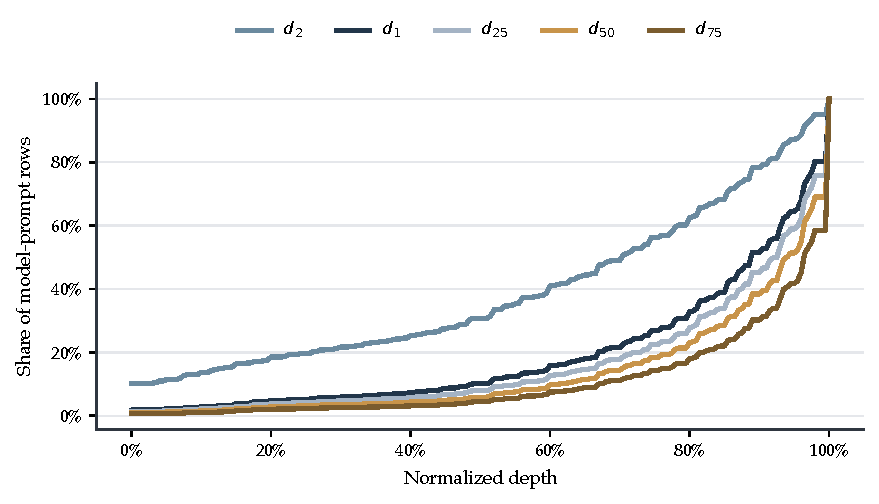
\includegraphics[width=\linewidth]{appendix_pooled_depths.pdf}
\caption{\textbf{Pooled CDFs including the appendix thresholds $d_{25}$ and $d_{75}$.} The same ordering remains visible when the margin threshold is relaxed or tightened.}
\end{figure}

\begin{figure}[h]
\centering
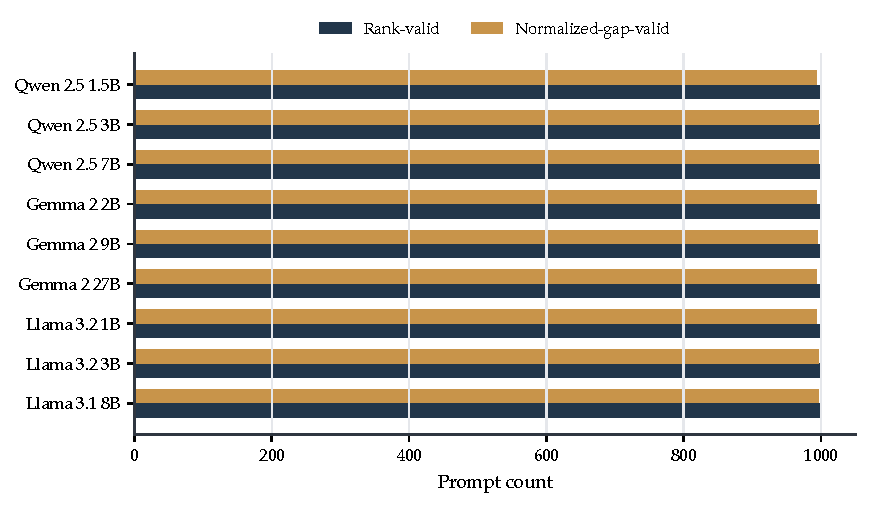
\includegraphics[width=0.92\linewidth]{appendix_valid_counts_by_model.pdf}
\caption{\textbf{Valid prompt counts by model.} Rank-based depths are available for all model-prompt rows. Normalized-gap analyses exclude only cases with a non-positive final gap.}
\end{figure}


\end{document}
